\section{Analyse}
In den folgenden Kapiteln, werden die punkte, welche bereits in der Themeneingabe
definiert wurden, präzisiert.

\subsection{Ausgangslage}
Um, als Indieentwickler, Projekte zu plaanen, hat man heutzutage bereits eine relativ grosse Auswahl an
Projektmanagement Tools.
Tools wie Azure DevOps sind jedoch hauptsächlich für grössere Teams gedacht und der mehraufwand schreckt die meisten Einzelentwickler ab.
Desshalb wird meisst auf ein Projektmanagement tool verzichtet und man behilft sich mit Post-Its oder einem Whiteboard.\\
Die meisten Projekt management Tools haben einen ähnlichen aufbau, welcher sich auch bewährt hat.
Um ein Produkt in dieser Kategorie zu entwickeln, ist es sicher eine gute Idee, bestehende Produkte etwas genauer anzusehen und vor und nachteile 
im bezug auf Indieentwickler rauszufiltern.

\subsubsection{Analyse von bestehenden Lösungen}


\begin{figure}[H]
    \begin{center}
        
\includegraphics[width=5cm]{../content/images/Trello/TrelloLogo.png}
        \caption{TRELLO Logo}
    \end{center}
\end{figure}

Trello ist ein Online-Tool zum verwalten von Aufgaben und gehört dem Unternehmen Atlassan. 
Das beliebte Online-Tool ist seit 2011 auf dem Markt und erfeut sich an milionen von Benutzern.


%------------------------------------------------------- 
%TRELLO BOARD SCREENSHOT
\begin{figure}[H]
    \begin{center}
        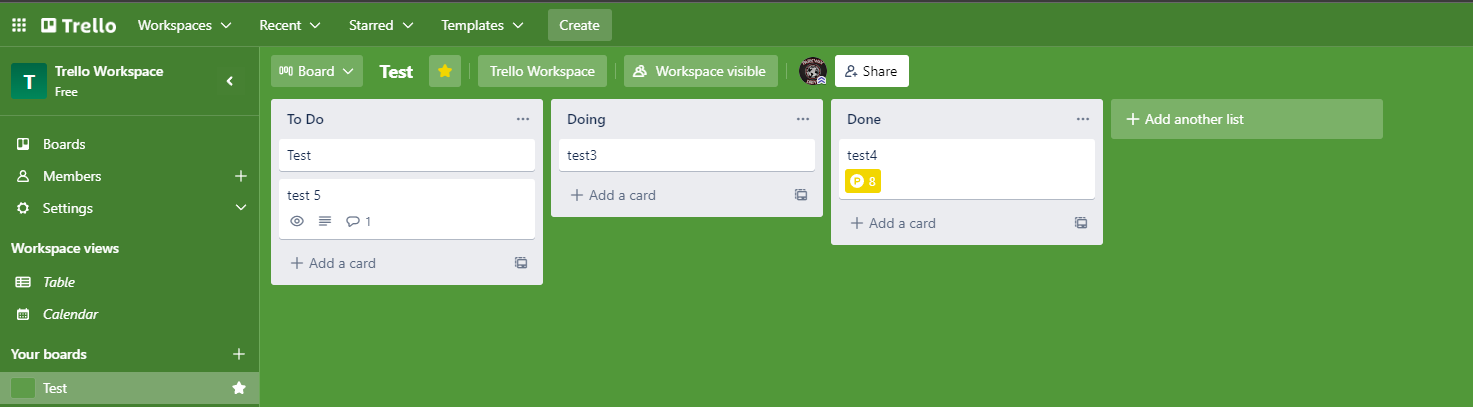
\includegraphics[width=16cm]{../content/images/Trello/TrelloBoard.png}
        \caption{TRELLO board}
    \end{center}
\end{figure}
%------------------------------------------------------- 

Das Layout entspricht einem klassischen Kanban-Board, welches jedoch nach belieben angepasst und
modifiziert werden kann. Das geschäftsmodell von trello lässt sich am ehsten als ''freemium'' bezeichen, die nötigsten Funktionen
sind gratis, reicht dies nicht aus, so kann ein Premium-Abo für 10.- pro monat abgeschlossen werden.
Beim Testen des Dienstes ist mir das penetrante anbieten des 30Days-Free-Trial angebotes, welche sich nach abschluss der 30 Tage automatisch verlängert
besonders negativ aufgefallen.\\
\space
%------------------------------------------------------- 
%TRELLO CARD SCREENSHOT WRAPPER
\begin{wrapfigure}{L}{0.4\textwidth}
    \begin{center}
        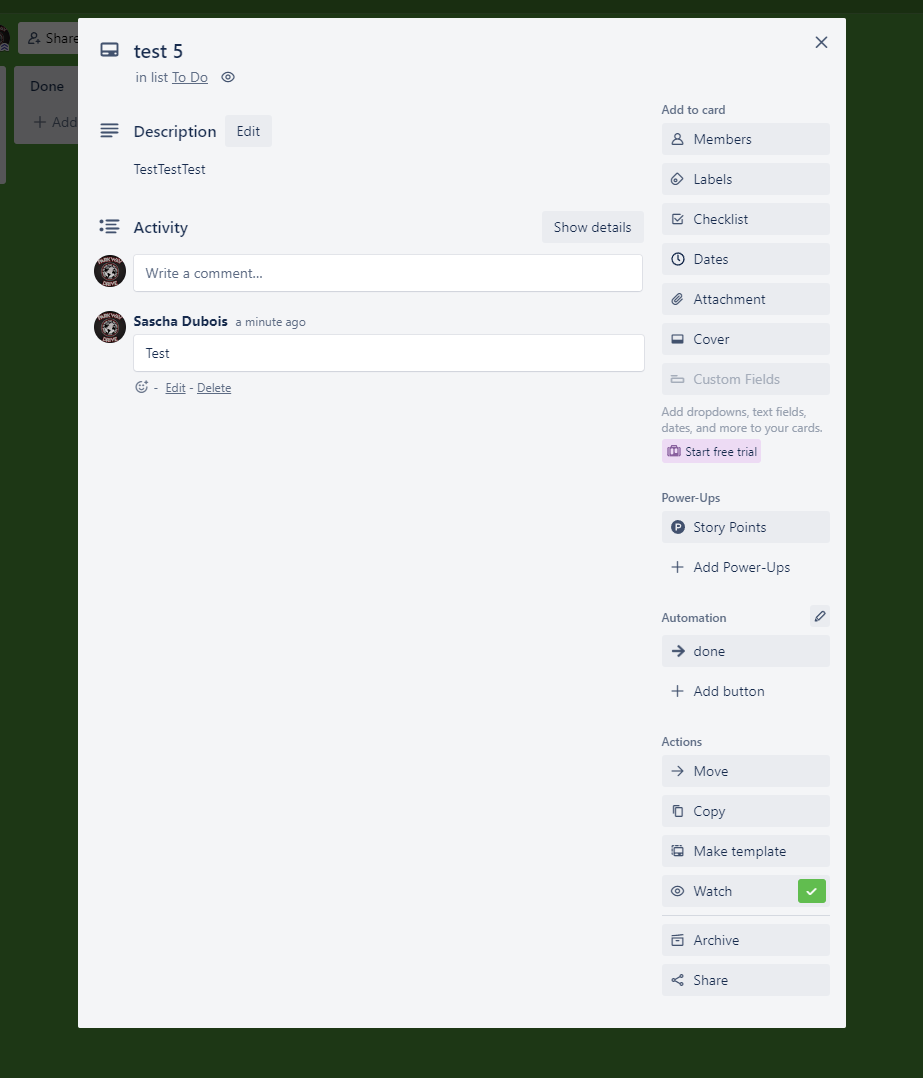
\includegraphics[width=5cm]{../content/images/Trello/TrelloCard.png}
        \caption{TRELLO Card}
    \end{center}
\end{wrapfigure}
%------------------------------------------------------- 

Dem Trello-Board können sogenannte ''Cards'' hinzugefügt werden. Den ''Cards'' kann man standartmässig
einen Titel, eine Beschreibung und Kommentare hinzufügen. Es lassen sich ausserdem
Personen, Labels, Checklists, Covers und Anhänge anfügen.\\
Fängt man das erste Projekt mit Trello an, so scheinen die Funktionen relativ übersichtlich zu sein.
Die grösste stärke, meiner Meinung nach, liegt jedoch in der konfigurierbarkeit von Trello. Es können nähmlich
''PowerUps'' eingefügt werden. PowerUps sind Plugins, mit denen die Funktionen von Trello beliebig erweitert werden können.
Zum Beispiel gibt es standartmässig keine möglichkeit den Cards irgendpwelche StoryPoints oder Stunden zuzuweisen.
Fügt man jedoch das entsprechende PowerUp hinzu so ist dies kein Problem mehr.\\
Und es gibt fast für alles ein entsprechendes PowerUp, so können auch Excel-Daten mittels PowerUp importiert werden.
Dem Benutzer sind also nur wehnig Grenzen gesetzt, was die Personalisierung von Trello angeht.\\

%------------------------------------------------------- 
%TRELLO POWERUPS SCREENSHOT WRAPPER
\begin{figure}[H]
    \begin{center}
        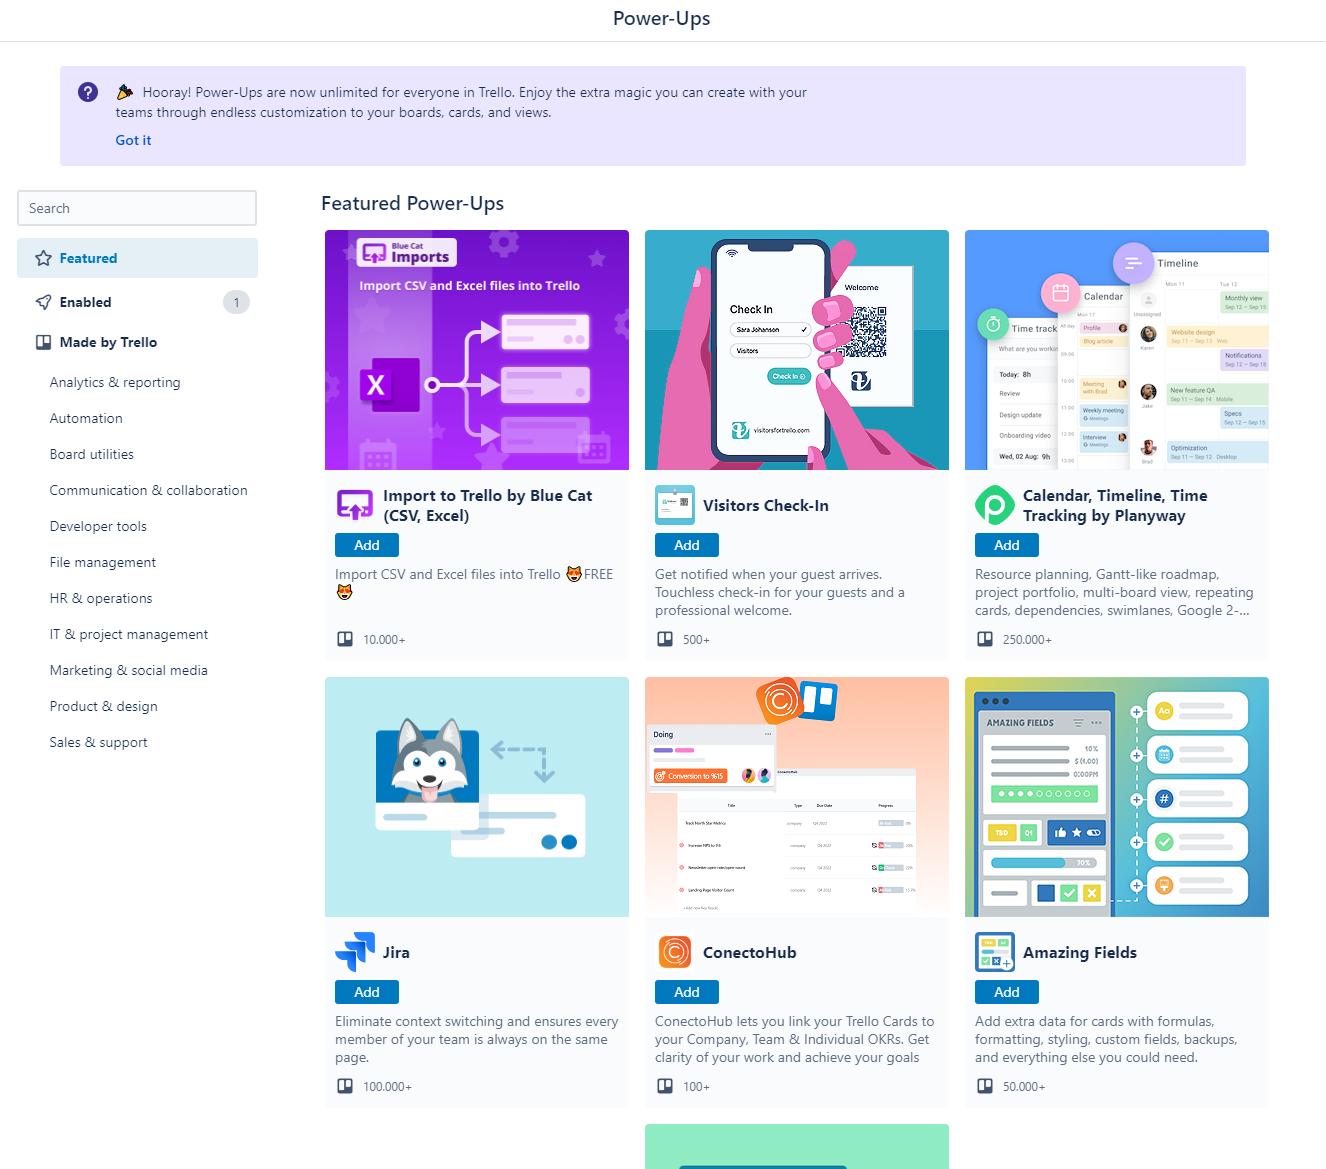
\includegraphics[width=8cm]{../content/images/Trello/PowerUps.png}
        \caption{TRELLO PowerUps}
    \end{center}
\end{figure}
%------------------------------------------------------- 

PowerUps können in einer art App-Store durchsucht und hinzugefügt werden.\\
Da die PowerUps auch von Trello-Usern erstellt werden können, gibt es fast für jeden Use-Case ein entsprechendes PowerUp
 
%------------------------------------------------------- 
%TRELLO DETAILS TABLE
\begin{table}[H]
    \centering
    \settowidth\tymin{executeIncomingCommand()}
    \setlength\extrarowheight{2pt}
    \begin{tabulary}{1.0\textwidth}{|L|L|}
      \hline
      \textbf{Besitzer} &
      Atlassan\\
      \hline
      \textbf{Gründung} &
      2011\\
      \hline
      \textbf{Plattform} &
      Web\\
      \hline
      \textbf{Layout} &
      Kanban\\
      \hline
      \textbf{Geschäftsmodell} &
      Freemium\\
      \hline
    \end{tabulary}
    \caption{TRELLO Details}
  \end{table}
%------------------------------------------------------- 

%------------------------------------------------------- 
%TRELLO RATING TABLE
\begin{table}[H]
    \centering
    \settowidth\tymin{executeIncomingCommand()}
    \setlength\extrarowheight{2pt}
    \begin{tabulary}{1.0\textwidth}{|L|L|L|}
      \hline
      \textbf{Bewertungspunkt} &
      \textbf{Bewertung} &
      \textbf{Begründung} \\
      \hline
      \textbf{Benutzerfreundlichkeit} &
      ****&
      Die Hohe konfigurierbarkeit führt zwangsläufig dazu, dass die Übersichtlichkeit der Funktionen etwas leidet\\
      \hline
      \textbf{Darstellung} &
      *****&
      Klassisches Kanbanboard, Backgrounds und Design können nach belieben angepasst werden\\
      \hline
      \textbf{Usability} &
      *****&
      Da Trello eine Webapplikation ist, ist sie auf allen webfähigen Geräten zugänglich\\
      \hline
      \textbf{Funktionalität} &
      *****&
      Durch die PowerUps kann die Funktionalität nach belieben erweitert werden\\
      \hline
      \textbf{Preis} &
      ****&
      Die Gratisversion ist absolut ausreichend, jedoch wird man immer wieder dazu gedrängt ein Premium-Abo abzuschliessen welches nicht gerade günstig ist\\
      \hline
    \end{tabulary}
    \caption{TRELLO Bewertung}
  \end{table}
%------------------------------------------------------- 
\space
\textbf{Punkte zur berücksichtigung in eigenem Projekt:}
\begin{itemize}
    \item Konfigurierbarkeit mittels anfügbarer Komponenten (PowerUps)
    \item Kanban Layout
    \item Design
\end{itemize}

  
  
\newpage

\begin{figure}[H]
    \begin{center}
        
\includegraphics[width=5cm]{../content/images/monday.com/MondayLogo.png}
        \caption{Monday.com Logo}
    \end{center}
\end{figure}

Monday.com ist eine Online-Plattform zum erstellen von Anwendungen und Arbeitsverwaltungs Software.
Die Plattform wurde 2014 veröffentlicht.

%------------------------------------------------------- 
%TRELLO BOARD SCREENSHOT
\begin{figure}[H]
    \begin{center}
        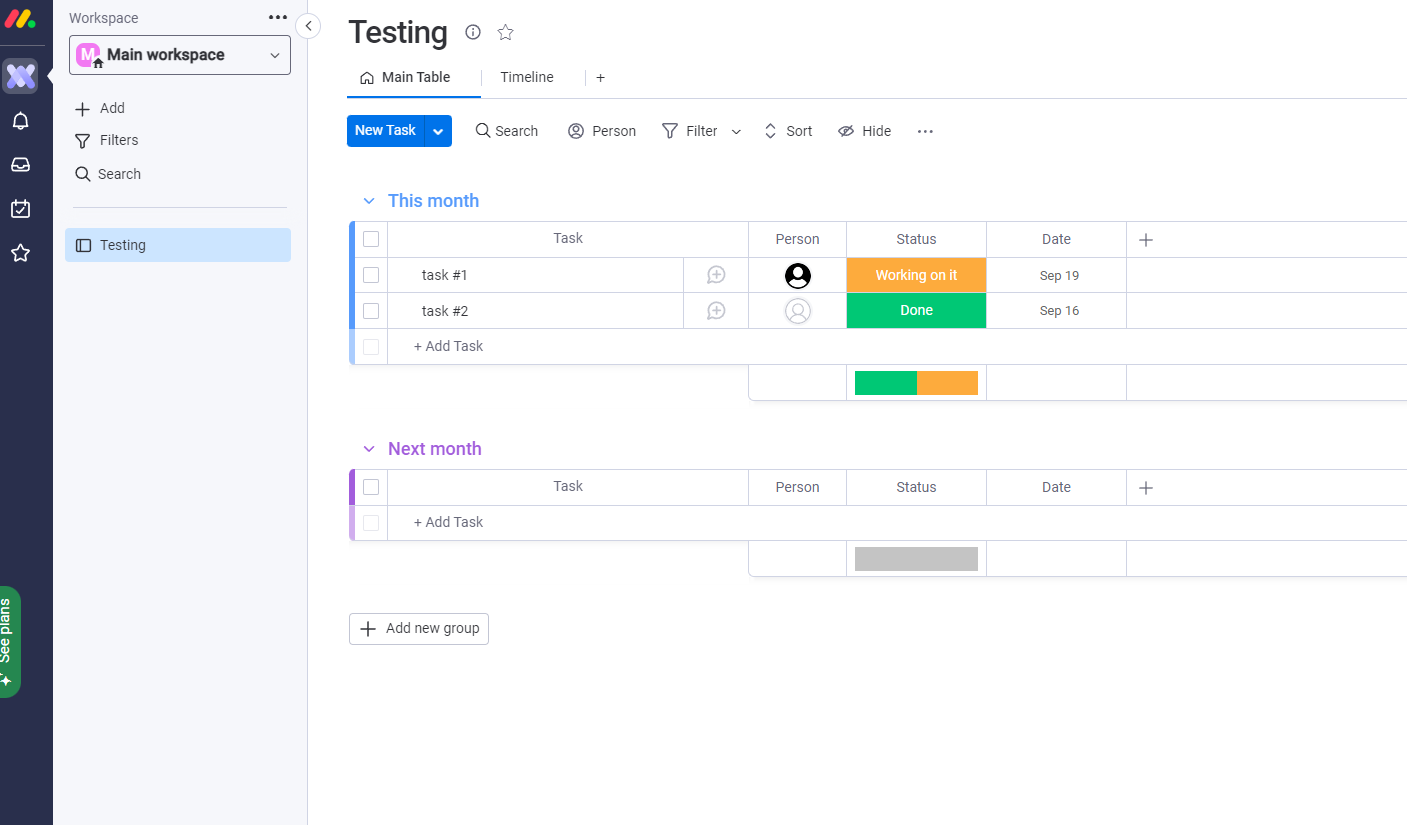
\includegraphics[width=16cm]{../content/images/monday.com/MondayBoard.png}
        \caption{TRELLO board}
    \end{center}
\end{figure}
%------------------------------------------------------- 

In der Standartkonfiguration werden Tasks aufgelistet und nicht als Kanbanboard dargestellt.
Wird ein neuer Workspace erstellt, so klickt man sich erst durch eine Reihe fragen, deren Resultate anschliessend das Layout und die Funktionen
des Workspaces vordefinieren.\\
Die Ansicht des Workspaces ist nach belieben konfigurierbar, so können  Tasks nach Monaten gruppiert werden oder aber auch zB. nach Sprints oder Thema.
Monday.com setzt ebenfalls auf das Freemium Geschäftsmodell, für ein Abo wird jedoch nicht so penetrant geworben wie bei anderen Anbietern.\\
\space
%------------------------------------------------------- 
%TRELLO CARD SCREENSHOT WRAPPER
\begin{figure}[H]
    \begin{center}
        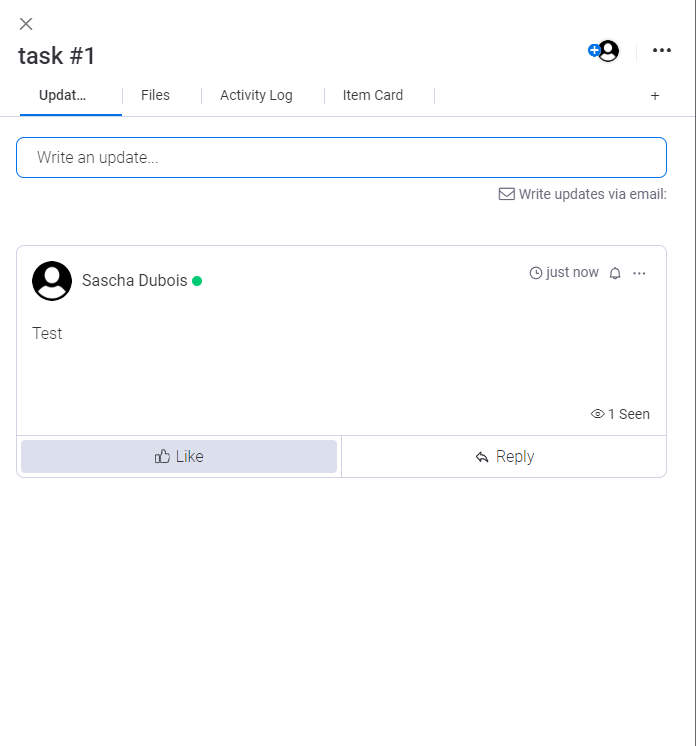
\includegraphics[width=5cm]{../content/images/monday.com/MondayTask.png}
        \caption{Monday.com Task}
    \end{center}
\end{figure}
%------------------------------------------------------- 

Monday.com können Tasks erstellt werden, im gegensatz zu anderen Anbietern sind diese Tasks
sehr minimalistisch gehalten und enthalten lediglich einen Titel und eine Beschreibung.\\
Den Tasks können jedoch weitere Views angefügt werden, in deren weiter felder und Funktionen zu verfügung stehen.
Vom Prinzip her gleicht es zwar den PowerUps von trello, dort finde ich jedoch die Anbindung um einiges
intuitiver und effizienter.\\

%------------------------------------------------------- 
%TRELLO POWERUPS SCREENSHOT WRAPPER
\begin{figure}[H]
    \begin{center}
        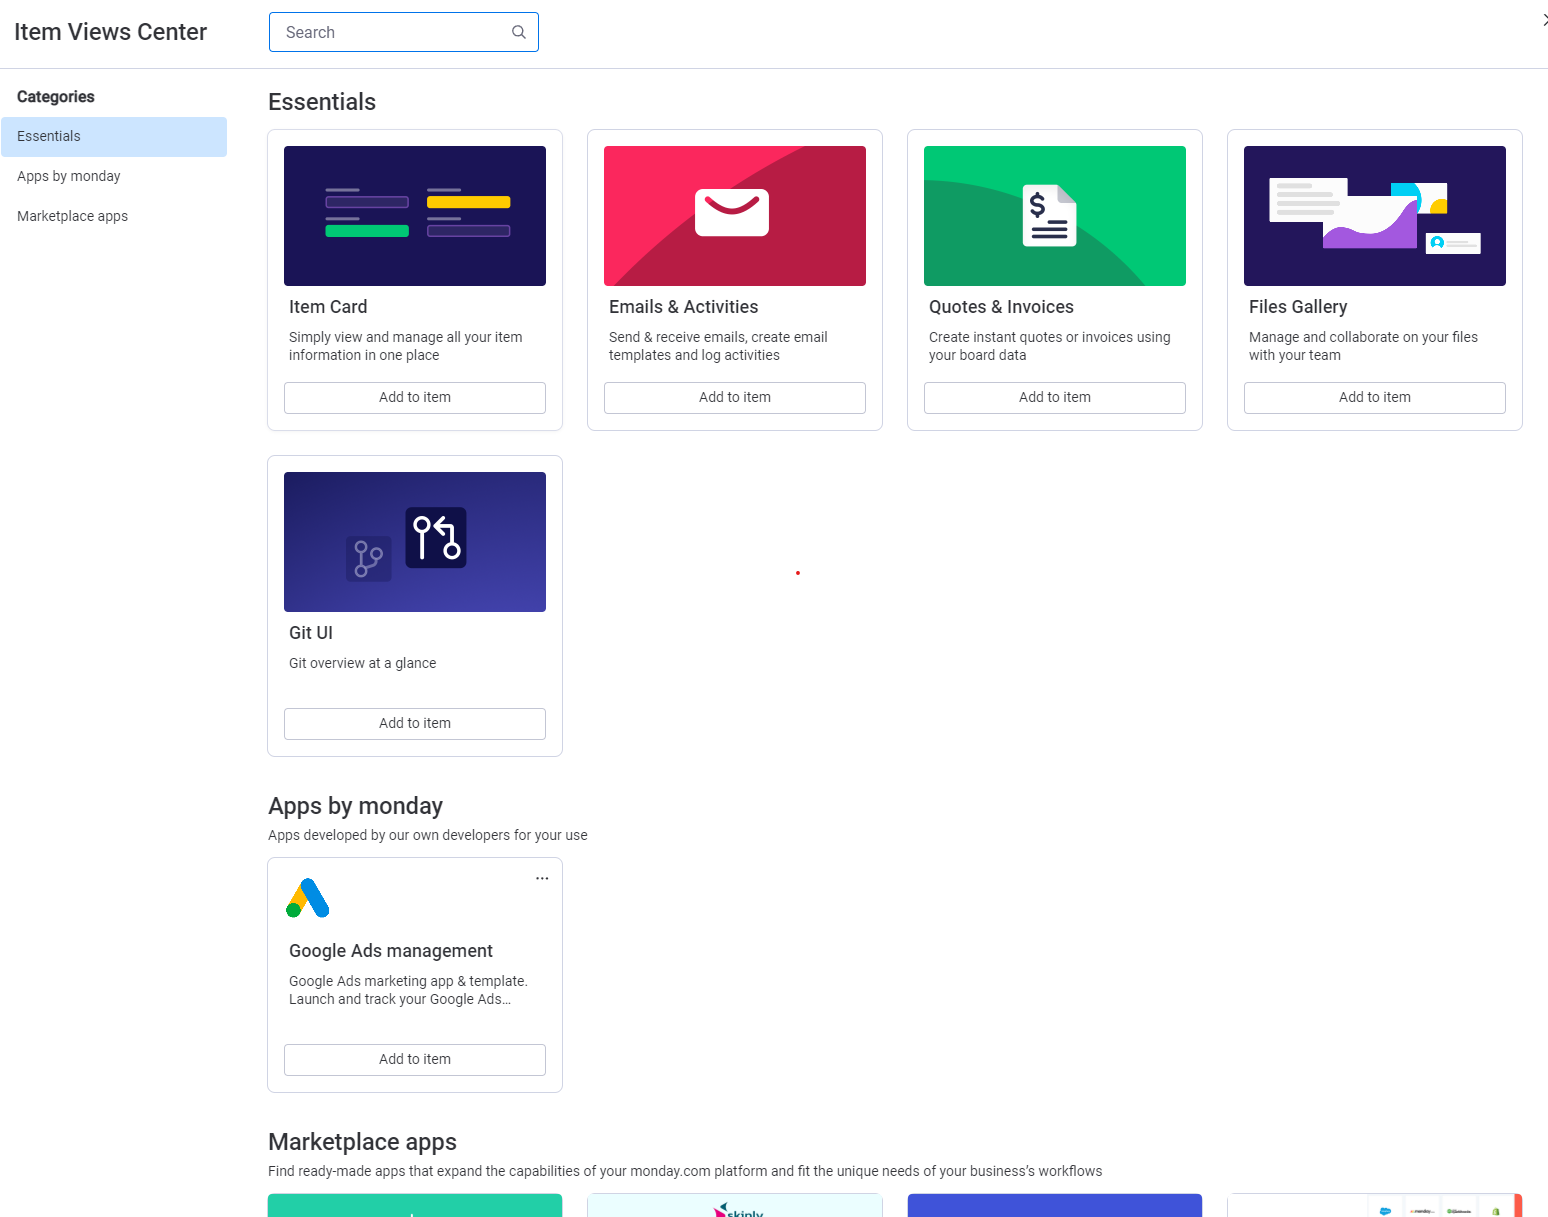
\includegraphics[width=8cm]{../content/images/monday.com/MondayItemViewsCenter.png}
        \caption{Monday.com Views}
    \end{center}
\end{figure}
%------------------------------------------------------- 

Views können im Item-View-Center durchstöbert und hinzugefügt werfden. 
Die hinzugefügten Views erscheinen dann in einem separaten Tab im Task. In den Views ist es ausserdem möglich Widgets einzufügen
und das generelle Layout zu konfigurieren.\\
Im Item-View-Center findet man native Monday.com Views aber auch ausreichend andere Views von drittanbietern.

%------------------------------------------------------- 
%TRELLO DETAILS TABLE
\begin{table}[H]
    \centering
    \settowidth\tymin{executeIncomingCommand()}
    \setlength\extrarowheight{2pt}
    \begin{tabulary}{1.0\textwidth}{|L|L|}
      \hline
      \textbf{Besitzer} &
      monday.com\\
      \hline
      \textbf{Gründung} &
      2012\\
      \hline
      \textbf{Plattform} &
      Web\\
      \hline
      \textbf{Layout} &
      Liste\\
      \hline
      \textbf{Geschäftsmodell} &
      Freemium\\
      \hline
    \end{tabulary}
    \caption{Monday.com Details}
  \end{table}
%------------------------------------------------------- 

%------------------------------------------------------- 
%TRELLO RATING TABLE
\begin{table}[H]
    \centering
    \settowidth\tymin{executeIncomingCommand()}
    \setlength\extrarowheight{2pt}
    \begin{tabulary}{1.0\textwidth}{|L|L|L|}
      \hline
      \textbf{Bewertungspunkt} &
      \textbf{Bewertung} &
      \textbf{Begründung} \\
      \hline
      \textbf{Benutzerfreundlichkeit} &
      ***&
      --\\
      \hline
      \textbf{Darstellung} &
      ****&
     Listenansichten werden schnell unübersichtlich\\
      \hline
      \textbf{Usability} &
      *****&
      Da monday.com eine Webapplikation ist, ist sie auf allen webfähigen Geräten zugänglich + gut optimiert für Mobilgeräte\\
      \hline
      \textbf{Funktionalität} &
      ****&
      Durch Views können Funktionalitäten hinzugefügt werden jedoch ist die auswahl deutlich kleiner als z.B. bei Trello\\
      \hline
      \textbf{Preis} &
      *****&
      Gratis version reicht vollkommen\\
      \hline
    \end{tabulary}
    \caption{Monday.com Bewertung}
  \end{table}
%------------------------------------------------------- 
\space
\textbf{Punkte zur berücksichtigung in eigenem Projekt:}
\begin{itemize}
    \item Lieber keine Listenansicht verwenden
\end{itemize}

  
  
\newpage

\subsection{Stakeholder}

\begin{itemize}
    \item TEKO
    \item Indieentwickler
    \item Konsumenten von Indiespielen
    \item Ich
    \item GitHub
    \item Unity
\end{itemize}


\newpage
\subsection{Ziele}
\newpage
\subsection{Anforderungen}
\newpage
\subsection{Abgrenzung}
\newpage
\subsection{Risikomanagement}
\newpage
\subsection{Wirtschaftlichkeit}